\documentclass[size=a4, parskip=half, titlepage=false, toc=flat, toc=bib, 12pt]{scrartcl}

\setuptoc{toc}{leveldown}

% Ajuste de las líneas y párrafos
\linespread{1.2}
\setlength{\parindent}{0pt}
\setlength{\parskip}{12pt}

% Español
\usepackage[spanish, es-tabla]{babel}

% Matemáticas
\usepackage{amsmath}
\usepackage{amsthm}

% Links
%\usepackage{hyperref}

% Fuentes
\usepackage{newpxtext,newpxmath}
\usepackage[scale=.9]{FiraMono}
\usepackage{FiraSans}
\usepackage[T1]{fontenc}

% \defaultfontfeatures{Ligatures=TeX,Numbers=Lining}
\usepackage[activate={true,nocompatibility},final,tracking=true,factor=1100,stretch=10,shrink=10]{microtype}
\SetTracking{encoding={*}, shape=sc}{0}

\usepackage{graphicx}
\usepackage{float}

% Mejores tablas
\usepackage{booktabs}

\usepackage{adjustbox}

% COLORES

\usepackage{xcolor}

\definecolor{verde}{HTML}{007D51}
\definecolor{esmeralda}{HTML}{045D56}
\definecolor{salmon}{HTML}{FF6859}
\definecolor{amarillo}{HTML}{FFAC12}
\definecolor{morado}{HTML}{A932FF}
\definecolor{azul}{HTML}{0082FB}
\definecolor{error}{HTML}{b00020}

% ENTORNOS
\usepackage[skins, listings, theorems]{tcolorbox}

\newtcolorbox{recuerda}{
  enhanced,
%  sharp corners,
  frame hidden,
  colback=black!10,
	lefttitle=0pt,
  coltitle=black,
  fonttitle=\bfseries\sffamily\scshape,
  titlerule=0.8mm,
  titlerule style=black,
  title=\raisebox{-0.6ex}{\small RECUERDA}
}

\newtcolorbox{nota}{
  enhanced,
%  sharp corners,
  frame hidden,
  colback=black!10,
	lefttitle=0pt,
  coltitle=black,
  fonttitle=\bfseries\sffamily\scshape,
  titlerule=0.8mm,
  titlerule style=black,
  title=\raisebox{-0.6ex}{\small NOTA}
}

\newtcolorbox{error}{
  enhanced,
%  sharp corners,
  frame hidden,
  colback=error!10,
	lefttitle=0pt,
  coltitle=error,
  fonttitle=\bfseries\sffamily\scshape,
  titlerule=0.8mm,
  titlerule style=error,
  title=\raisebox{-0.6ex}{\small ERROR}
}

\newtcblisting{shell}{
  enhanced,
  colback=black!10,
  colupper=black,
  frame hidden,
  opacityback=0,
  coltitle=black,
  fonttitle=\bfseries\sffamily\scshape,
  %titlerule=0.8mm,
  %titlerule style=black,
  %title=Consola,
  listing only,
  listing options={
    style=tcblatex,
    language=sh,
    breaklines=true,
    postbreak=\mbox{\textcolor{black}{$\hookrightarrow$}\space},
    emph={jmml@UbuntuServer, jmml@CentOS},
    emphstyle={\bfseries},
  },
}

\newtcbtheorem[number within=section]{teor}{\small TEOREMA}{
  enhanced,
  sharp corners,
  frame hidden,
  colback=white,
  coltitle=black,
  fonttitle=\bfseries\sffamily,
  %separator sign=\raisebox{-0.65ex}{\Large\MI\symbol{58828}},
  description font=\itshape
}{teor}

\newtcbtheorem[number within=section]{prop}{\small PROPOSICIÓN}{
  enhanced,
  sharp corners,
  frame hidden,
  colback=white,
  coltitle=black,
  fonttitle=\bfseries\sffamily,
  %separator sign=\raisebox{-0.65ex}{\Large\MI\symbol{58828}},
  description font=\itshape
}{prop}

\newtcbtheorem[number within=section]{cor}{\small COROLARIO}{
  enhanced,
  sharp corners,
  frame hidden,
  colback=white,
  coltitle=black,
  fonttitle=\bfseries\sffamily,
  %separator sign=\raisebox{-0.65ex}{\Large\MI\symbol{58828}},
  description font=\itshape
}{cor}

\newtcbtheorem[number within=section]{defi}{\small DEFINICIÓN}{
  enhanced,
  sharp corners,
  frame hidden,
  colback=white,
  coltitle=black,
  fonttitle=\bfseries\sffamily,
  %separator sign=\raisebox{-0.65ex}{\Large\MI\symbol{58828}},
  description font=\itshape
}{defi}

\newtcbtheorem{ejer}{\small EJERCICIO}{
  enhanced,
  sharp corners,
  frame hidden,
  left=0mm,
  right=0mm,
  colback=white,
  coltitle=black,
  fonttitle=\bfseries\sffamily,
  %separator sign=\raisebox{-0.65ex}{\Large\MI\symbol{58828}},
  description font=\itshape,
  nameref/.style={},
}{ejer}

% CÓDIGO
\usepackage{listings}

% CABECERAS
\pagestyle{headings}
\setkomafont{pageheadfoot}{\normalfont\normalcolor\sffamily\small}
\setkomafont{pagenumber}{\normalfont\sffamily}

% ALGORITMOS
\usepackage[vlined,linesnumbered]{algorithm2e}
\usepackage{listings}
\usepackage{color}
\renewcommand{\lstlistingname}{Listado}

\definecolor{dkgreen}{rgb}{0,0.6,0}
\definecolor{gray}{rgb}{0.5,0.5,0.5}
\definecolor{mauve}{rgb}{0.58,0,0.82}

\lstset{frame=tb,
  language=Python,
  aboveskip=3mm,
  belowskip=3mm,
  showstringspaces=false,
  columns=flexible,
  basicstyle={\small\ttfamily},
  numbers=none,
  numberstyle=\tiny\color{gray},
  keywordstyle=\color{blue},
  commentstyle=\color{dkgreen},
  stringstyle=\color{mauve},
  breaklines=true,
  breakatwhitespace=true,
  tabsize=2
}

% Formato de los pies de figura
\setkomafont{captionlabel}{\scshape}
\SetAlCapFnt{\normalfont\scshape}
\SetAlgorithmName{Algoritmo}{Algoritmo}{Lista de algoritmos}

% BIBLIOGRAFÍA
%\usepackage[sorting=none]{biblatex}
%\addbibresource{bibliografia.bib}

\begin{document}

\renewcommand{\proofname}{\normalfont\sffamily\bfseries\small DEMOSTRACIÓN}

\title{Proyecto final}
\subject{Aprendizaje automático}
\author{Johanna Capote Robayna\\
Guillermo Galindo Ortuño \\
    5 del Doble Grado en Informática y Matemáticas\\
    Grupo A}
\date{}
\publishers{\vspace{2cm}
\includegraphics[height=2.5cm]{UGR}\vspace{1cm}}
\maketitle

\newpage

\tableofcontents
\newpage

\section{Definición del problema a resolver y enfoque elegido}

El problema que inicialmente se nos plantea es del estimar la popularidad de un artículo (medido como número de veces que este es compartido) basándonos en una serie de características de este, como por ejemplo la longitud o si trata de temas como tecnología, estilo de vida, etc.

Aunque lo natural sería haberlo plantearlo como un problema de regresión, en nuestro caso hemos decidido enfocarlo como un problema de clasificación binario. Esto lo hemos hecho para poder utilizar y analizar modelos de clasficación tal y como hemos estudiado, que creemos que será más interesante. Siguiendo las recomendaciones de los creadores de la base de datos, trataremos este problema como un problema de clasificación binaria, considerando todos aquellos valores del atributo objetivo menores o iguales que un umbral ($1400$ en particular) como una clase y los mayores como la otra. Esto podemos interpretarlo como que queremos conocer si un artículo será popular  o no (supera o no el umbral de \textit{shares}).

El \textit{dataset} consta de 61 atributos, siendo dos de ellos no predictivos  (\textit{url} y \textit{timedelta}) y otro distinto el objetivo. Por tanto nuestro vector de características tendrá será de tamaño 58. Formalmente:
\begin{itemize}
\item Nuestro espacio muestral será $ \mathcal{X}= \mathbb{R}^{58}$.
\item El espacio de etiquetas será $\mathcal{Y}: \{-1,1\}$.
\item Nuestro objetivo será encontrar $f:X \rightarrow Y$ que estime si un artículo será popular o no (\(1\) ó \(-1\)).
\end{itemize}

\section{Argumentos a favor de la elección de los modelos}

\section{Codificación de los datos de entrada par hacerlo útiles a los algoritmos}
En priner lugar, tras quitar los atributos no predicitivos (\verb|url| y \verb|timedelta|),comprobamos que no hay valores perdidos y que ninguno sea \textit{null}:
\begin{verbatim}
datos_perdidos = datos.columns[datos.isnull().any()]
datos_perdidos = datos.columns[datos.isna().any()]
\end{verbatim}
A continuación dividimos el \textit{dataset} en el conjunto de características y el conjunto de etiquetas. Y transformamos las etiquetas asignándole el valor $-1$ si la etiqueta tiene un valor menor que $1400$ y asignándole el valor $1$ en el otro caso.
\begin{verbatim}
datos_perdidos = datos.columns[datos.isnull().any()]
datos_perdidos = datos.columns[datos.isna().any()]
y = y.apply(lambda x: -1.0 if x < 1400 else 1.0)
\end{verbatim}

Por último antes de pasar al preprocesado de los datos comprobamos que los valores se encuentran dentro del rango. El valor mínimo es $-1.0$ y el valor máximo es $843300.0$, por lo que no hay valores fuera de rango. Además comprobamos que las clases están balanceadas.
\begin{figure}[H]
\centering
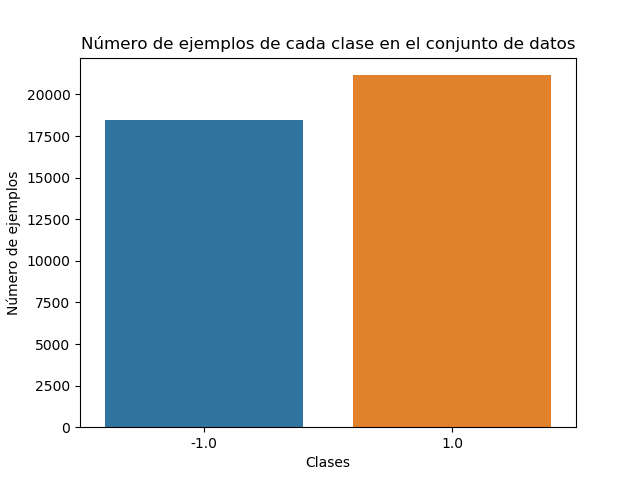
\includegraphics[width=1\textwidth]{./img/balanceadas}
\caption{Gráfica que muestra el número de individuos de cada clase.}
\end{figure}

Dividimos el conjunto de datos en el conjunto de entrenamiento y el conjunto de test, para ello utilizamos la función \verb|train_test_split()| de la librería \textit{sklearn}. Elegimos que el conjunto de test tenga un tamaño del $20\%$, medida estándar.

Para preprocesar los datos utilizamos una estructura \verb|Pipeline| de \texit{sklearn} para agrupar todas las transformaciones. Realizamos dos transformaciones de los datos:
\begin{enumerate}
\item En primer lugar utilizamos la transformación \verb|StandardScaler()| para reescalar los atributos para evitar datos con distintas escalas. Tras estre reescalado los atributos tienen media $0$ y varianza $1$. Realizamos esta transformación ya que es altamente recomendable que se realice antes de entrenar los modelos que hemos elegido.

\item Además aplicamos el algoritmo PCA, con el conseguimos reducir la dimensionalidad de las características. Se ha fijado que seleccione el número de componentes de modo que la cantidad de varianza que deba explicarse sea mayor del $95\%$. Elegimos aplicar esta transformación puesto que la cantidad de atributos es considerablemente grande, con ella buscamos mejorar la eficiencia de los modelos y encontrar una base de coordenadas que sea más representativa (eliminando las correlaciones entre los atributos), hallando aquellas características con mayor relevancia.

\end{enumerate}
Por lo que el Pipeline del preprocesador quedaría de la siguiente forma:
\begin{verbatim}
preprocesado = [("escalado", StandardScaler()),
                ("PCA", PCA(n_components=0.95))]

preprocesador = Pipeline(preprocesado)
\end{verbatim}
Para analizar los logros obtenidos con el preprocesado de datos utilizamos una matriz de correlaciones con la que podemos observar que el preprocesador de datos ha mejorado la correlación de las características. En las siguientes imágenes podemos observar como se ha reduciendo a 35 las características y se han eliminado las correlaciones entre ellas.
\begin{figure}[H]
\centering
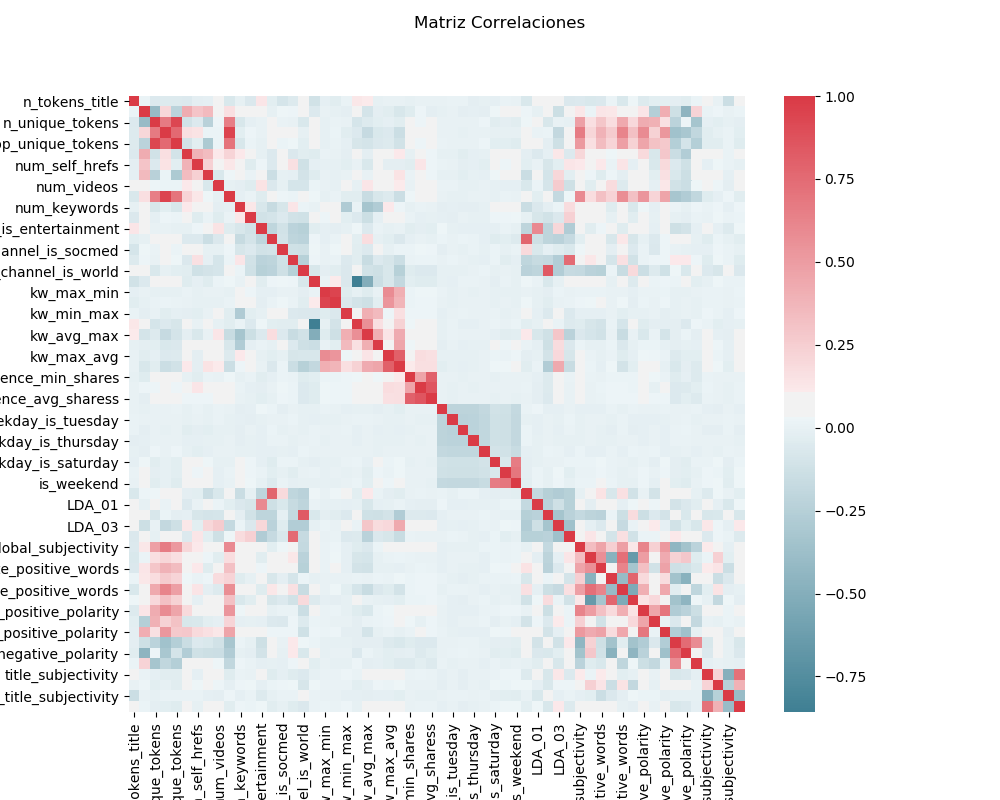
\includegraphics[width=1\textwidth]{./img/antespre}
\caption{Matriz de correlaciones antes del preprocesador de datos.}
\end{figure}
\begin{figure}[H]
\centering
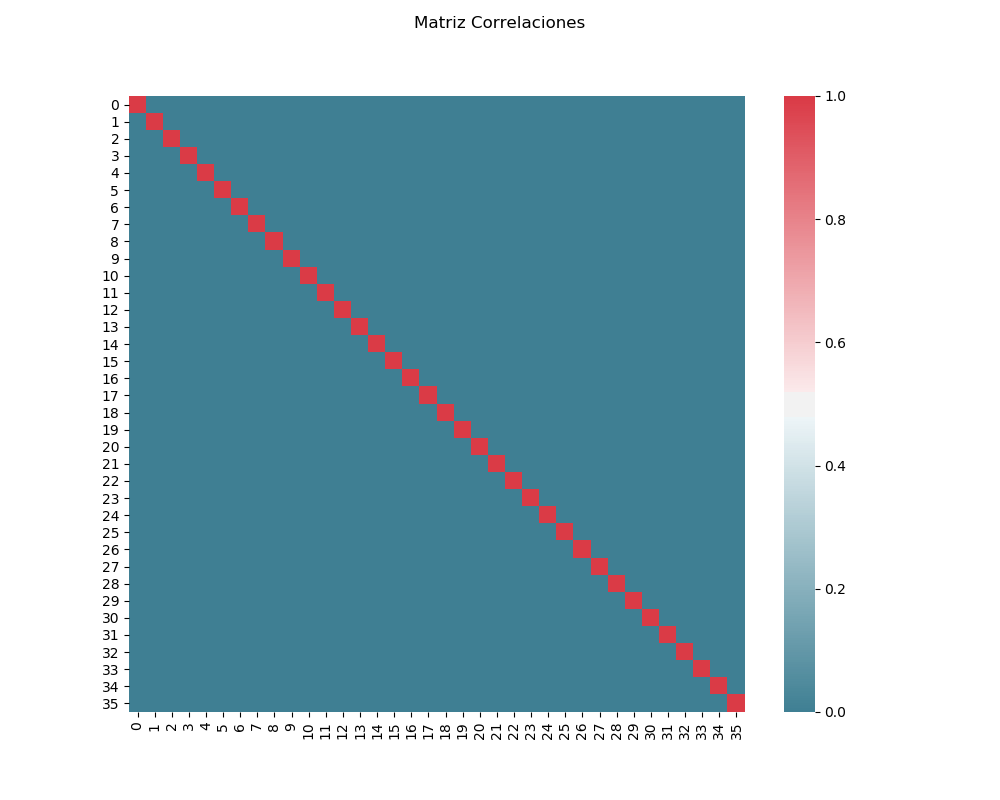
\includegraphics[width=1\textwidth]{./img/despuespre}
\caption{Matriz de correlaciones después del preprocesado de datos.}
\end{figure}

\section{Valoración del interés de las variables para el problema y selección de un subconjunto}
\section{Normalización de las variables}
\section{Justificación de la función de pérdida usada}
Como métrica de error utilizaremos el \textit{accuracy}, la usual en este tipo de problemas. Esta medida expresa el error como un valor entre 0 y 1, siendo 0 cuando todos los puntos están bien clasificados y 1 cuando están todos mal clasificados. Para calcularla, dado un $h \in H$ el error viene dado por:
$$E_{in}(h) = \frac{1}{N} \sum_{x_n \in X} [[ h(x) \neq y_n]] $$

Para visualizar y analizar el error utilizamos la matriz de confusión, aunque está no es una medida métrica, la mayoría de métricas se basan en esta matriz. Esta matriz es un método visual en el que podemos ver el rendimiento de un modelo supervisado. Esta matriz muestra los falsos positivos y los verdaderos positivos.
\section{Selección del modelo lineal paramétrico y valoración de su idoneidad frente a otras alternativas}

Para seleccionar el mejor modelo utilizamos la función \verb|GridSearchCV| la cual utiliza la técnica de \textit{cross-validation} para entrenar y validar los distintos modelos. Esta función elabora un grid con todas las posibles combinaciones de los diccionarios sin mezclar entre ellos (cada estimador con sus parámetros),por lo que le pasamos el preprocesador y la lista con todos los modelos a probar. A continuación entrenamos el \textit{grid} con la función \verb|fit| y elegimos como nuestro clasificador final el mejor estimador, el cual será el que tenga mejor \textit{accuracy}. Este estimador que nos devuelve el \verb|GridSearchCV| ya está entrenado en todo el conjunto de entrenamiento por lo que no es necesario volverlo a entrenar.
\begin{verbatim}
grid = GridSearchCV(preprocesador, modelos, scoring='accuracy', cv=5,
                    n_jobs = -1)
grid.fit(X, y)
clasificador = grid.best_estimator_
\end{verbatim}

Tras ejecutar esto con nuestra lista de modelos, obtenemos como resultado que el mejor clasificador es la combinación del estimador ?? y el parámetro ??.

\section{Aplicación de técnicas}
\section{Función de regularización}
Para evitar sobreajustes en el modelo debido a la alta dimensión de nuestro conjunto de datos introducimos técnicas de regularización, las cuales reducen la complejidad de modelo introduciendo un término en la función de coste. Es decir, la regularización reduce la varianza del modelo sin incrementar considerablemente el sesgo de este.

Dentro de todos los métodos de regularización, elegimos la Regularización de Ridge($L_2$) ya que proporciona mejores resultados cuando la mayoría de los atributos son relevantes, como es nuestro caso.

Este método añade una penalización cuadrática en los pesos a la función de pérdida (L):
$$L_{(L_2)}(w) = L(w) + \lambda \|w\|_2^2 $$

\section{Valoración de los resultados}
\section{Justificación}

%printbibliography

\end{document}
